\documentclass[8pt]{beamer}
\usepackage{csvsimple}
\usepackage{subcaption}
\graphicspath{{./images/}}

\newcommand{\csvloopx}[2][]{\csvloop{#1,#2}}
\newcommand{\csvautotabularx}[2][]{\csvloopx[#1]{autotabular={#2}}}
\newcommand{\respectpercent}{\catcode`\%=12\relax}

\newcommand{\resultsframe}[1]
{
\begin{frame}
 \frametitle{#1}
 \begin{center}
  \csvreader[tabular=|l|l|l|,before table=\respectpercent, no head,column count=3, table head=\hline,late after line=\\\hline]{#1.csv}{}{\csvlinetotablerow}
 \end{center}
 
 \begin{columns}
  \begin{column}{0.3\textwidth}
   \includegraphics[height=0.2\textheight]{#1Coronal0.png} \\
   \includegraphics[height=0.2\textheight]{#1Coronal1.png} \\
   \includegraphics[height=0.2\textheight]{#1Coronal2.png} \\
  \end{column}
  \begin{column}{0.2\textwidth}
   \includegraphics[height=0.2\textheight]{#1Axial0.png} \\
   \includegraphics[height=0.2\textheight]{#1Axial1.png} \\
   \includegraphics[height=0.2\textheight]{#1Axial2.png} \\    
  \end{column}
  \begin{column}{0.3\textwidth}
   \includegraphics[height=0.2\textheight]{#1Sagittal0.png} \\
   \includegraphics[height=0.2\textheight]{#1Sagittal1.png} \\
   \includegraphics[height=0.2\textheight]{#1Sagittal2.png} \\
  \end{column}
 \end{columns}
\end{frame}
}

\begin{document}
 \begin{frame}
  \frametitle{Explanation}
  \begin{itemize}
   \item \emph{Checkerbording} is a technique used to evaluate the image registration quality.
    It is analogous to placing the deformed registered (moving) image on the red squares and the target (fixed) image on the black squares of a checkerboard.
    If the registration quality is high structures will be aligned across squares.
    The ITK documentation has a good example of it's usage: \\ 
    \tiny{\url{https://itk.org/ITKExamples/src/Registration/Common/PerformMultiModalityRegistrationWithMutualInformation/Documentation.html}}

   \item The first, second and third columns of the following sildes are CLARITY-ARA checkerboard images of selected coronal, axial and sagittal slices.
    \begin{figure}
     \begin{subfigure}{0.30\textwidth}
      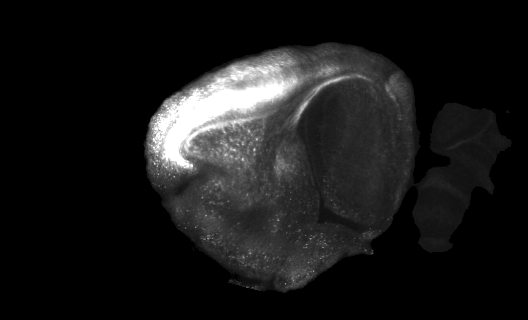
\includegraphics[width=\textwidth]{clarity.png}
      \caption{CLARITY}
     \end{subfigure}
     \begin{subfigure}{0.30\textwidth}
      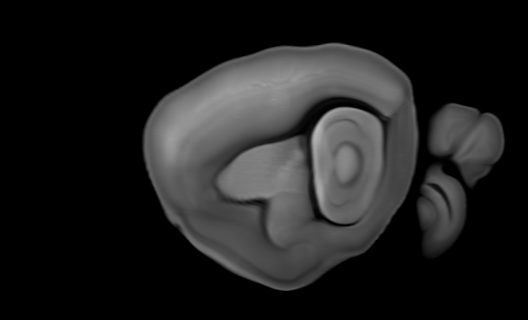
\includegraphics[width=\textwidth]{ara.png}
      \caption{Atlas}
     \end{subfigure}
     \begin{subfigure}{0.30\textwidth}
      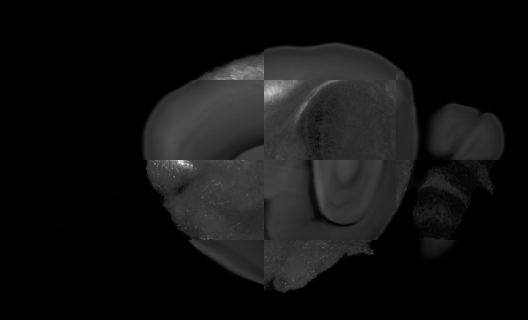
\includegraphics[width=\textwidth]{checker.png}
      \caption{Checkerboard}
     \end{subfigure}
    \end{figure}
  \end{itemize}
 \end{frame}

 \begin{frame}
  \begin{itemize}
   \item Many CLARITY images are missing data thus the corresponding checkerboard images have empty squares
    \begin{figure}
     \begin{subfigure}{0.30\textwidth}
      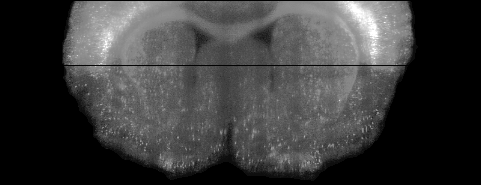
\includegraphics[width=\textwidth]{missingData.png}
      \caption{CLARITY image missing superior portion of brain}
     \end{subfigure}
     \begin{subfigure}{0.30\textwidth}
      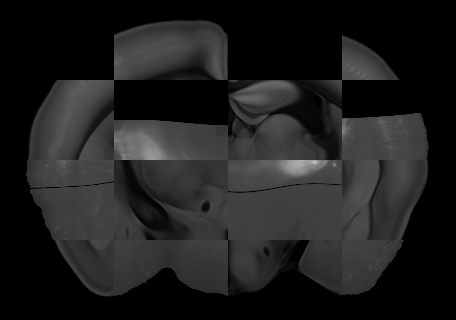
\includegraphics[width=\textwidth]{missingDataChecker.png}
      \caption{Checkerboard}
     \end{subfigure}
    \end{figure}
   \item For example registration of \textbf{Control182} worked despite missing data while \textbf{Control189} did not.
  \end{itemize}
 \end{frame}

 \begin{frame}
  For cost function $M$
  \begin{itemize}
   \item ``Value'' column contains $M(I_0 \circ \varphi_{01}, I_1)$
   \item ``Value (\%)'' column contins the normalized value.  Lower ``Value (\%)'' indicates a better match.
    \begin{equation*}
     \frac{M(I_0 \circ \varphi_{10}, I_1) - M(I_1, I_1)}{M(I_0, I_1) - M(I_1, I_1)} * 100\%
    \end{equation*}
  \end{itemize}
 \end{frame}

 \resultsframe{Cocaine174}
 \resultsframe{Cocaine175}
 \resultsframe{Cocaine178}
 \resultsframe{Control181}
 \resultsframe{Control182}
 \resultsframe{Control189}
 \resultsframe{Control239}
 \resultsframe{Control258}
 \resultsframe{Fear187}
 \resultsframe{Fear197}
 \resultsframe{Fear199}
\end{document}